% DRAFT slides for the deck's opening section: Table of Contents, Motivation and
% Problem, GFL/GFM explained as a DIAGRAM, and what the project delivers.
%
% WHY A SEPARATE FILE. This compiles on its own with the SAME preamble as
% docs/source/presentation_pf_sssa_ts_gfm_en_v11.tex, so the new slides can be
% rendered and judged before anything in the delivered deck is touched. Nothing
% here is wired into v11 yet.
%
% MERGE NOTES, so the integration is mechanical:
%   1. v11.tex:28 loads \usetikzlibrary{arrows.meta,positioning,shapes}. Every
%      diagram below uses only those three, so the line needs NO change.
%   2. v11 defines pnavy/pblue/pgreen/pred/pyellow (v11.tex:31-35) and \pu
%      (v11.tex:56); all are reused, none redefined.
%   3. The frames replace v11.tex:77-130 (Table of Contents, Introduction,
%      Project Objectives). The section names match the existing TOC entries, so
%      the hand-built TOC stays valid.
%   4. Language follows the delivered deck: English on the slide. v11 carries no
%      Thai and mixing one Thai slide into an English deck would read as an
%      accident rather than a choice.
%
% The GFL/GFM slide is a diagram rather than two bullet blocks because the
% distinction is structural, not a list of properties: one converter MEASURES an
% angle that already exists, the other IMPOSES one. A reader can see that in a
% signal path and cannot see it in prose.
\documentclass{beamer}
\usepackage{fontspec}
\setsansfont[Path=C:/Users/User/AppData/Local/Microsoft/Windows/Fonts/,UprightFont=Helvetica.ttf,BoldFont=Helvetica-Bold.ttf,ItalicFont=Helvetica-Oblique.ttf,BoldItalicFont=Helvetica-BoldOblique.ttf]{Helvetica.ttf}
\usetheme{Berlin}
\usefonttheme[onlymath]{serif}
\setbeamertemplate{footline}{%
  \leavevmode%
  \hbox{%
  \begin{beamercolorbox}[wd=.88\paperwidth,ht=2.6ex,dp=1.1ex,leftskip=1.2em]{author in head/foot}%
    \ifodd\insertframenumber\relax
      \scriptsize An Automatic Following/Forming Framework for Inverter-Based Resources%
    \else
      \scriptsize Department of Electrical Engineering, School of Engineering, KMITL%
    \fi
  \end{beamercolorbox}%
  \begin{beamercolorbox}[wd=.12\paperwidth,ht=2.6ex,dp=1.1ex,center]{date in head/foot}%
    \scriptsize \insertframenumber/\inserttotalframenumber
  \end{beamercolorbox}}%
}
\usepackage{xcolor}
\usepackage{graphicx}
\usepackage{amsmath,amsfonts,amssymb}
\usepackage{bm}
\usepackage{booktabs,array,multicol}
\usepackage{tikz}
\usetikzlibrary{arrows.meta,positioning,shapes}
\definecolor{myblue}{rgb}{0.0,0.0,0.7}
\definecolor{pnavy}{HTML}{0F2A4A}
\definecolor{pblue}{HTML}{1D5288}
\definecolor{pgreen}{HTML}{1E7E34}
\definecolor{pred}{HTML}{A93226}
\definecolor{pyellow}{HTML}{B7950B}
\setbeamercolor{item}{fg=myblue}
\setbeamercolor{block title}{bg=myblue,fg=white}
\setbeamercolor{block body}{bg=blue!7,fg=black}
\setbeamercolor{itemize item}{fg=myblue}
\setbeamertemplate{navigation symbols}{}
\setbeamercolor{frametitle}{bg=myblue!82!black,fg=white}
\setbeamertemplate{section in toc}[sections numbered]
\setbeamertemplate{background}{}
\setbeamertemplate{headline}{}
\newcommand{\pu}{\,\mathrm{p.u.}}
\begin{document}
% ===================== 1. TABLE OF CONTENTS ==============================
% Same hand-built tabular as v11.tex:77-88 (no \tableofcontents), same six
% entries, unchanged. Reproduced here only so the draft renders as a deck
% opening rather than a loose slide.
\begin{frame}{Table of Contents}
\centering
\renewcommand{\arraystretch}{1.65}
\begin{tabular}{c@{\hspace{0.35cm}}l}
\colorbox{myblue}{\makebox[0.52cm][c]{\color{white}\Large 1}} & {\Large Introduction and Motivation}\\
\colorbox{myblue}{\makebox[0.52cm][c]{\color{white}\Large 2}} & {\Large Project Objectives}\\
\colorbox{myblue}{\makebox[0.52cm][c]{\color{white}\Large 3}} & {\Large System Workflow and Case Study}\\
\colorbox{myblue}{\makebox[0.52cm][c]{\color{white}\Large 4}} & {\Large PF, SSSA and TS Formulation}\\
\colorbox{myblue}{\makebox[0.52cm][c]{\color{white}\Large 5}} & {\Large Dual-Mode IBR and Switching}\\
\colorbox{myblue}{\makebox[0.52cm][c]{\color{white}\Large 6}} & {\Large Results and Conclusions}
\end{tabular}
\end{frame}

% ===================== 2. WHY THIS PROJECT ===============================
% The motivation slide. One physical fact drives everything: a synchronous
% machine supplies the angle reference as a by-product of its rotating mass,
% and a converter does not. The diagram shows what the network loses when the
% machine leaves, which is the problem the rest of the deck answers.
\section{Introduction}
\begin{frame}{Why This Project: The Reference Disappears}
\centering
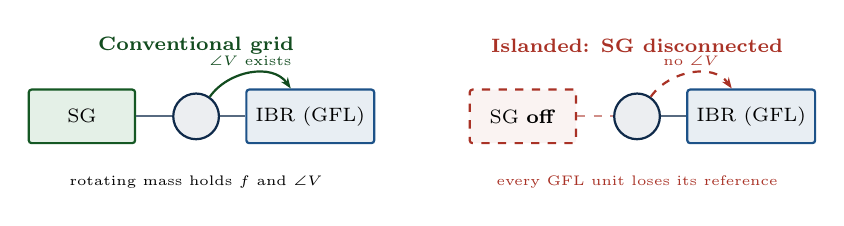
\begin{tikzpicture}[
  font=\scriptsize,
  bus/.style={circle,draw=pnavy,thick,fill=pnavy!8,minimum size=0.58cm,inner sep=0pt},
  mach/.style={draw=pgreen!70!black,thick,fill=pgreen!12,rounded corners=1pt,
               minimum width=1.35cm,minimum height=0.68cm,align=center},
  conv/.style={draw=pblue,thick,fill=pblue!10,rounded corners=1pt,
               minimum width=1.45cm,minimum height=0.68cm,align=center},
  gone/.style={draw=pred,thick,dashed,fill=pred!6,rounded corners=1pt,
               minimum width=1.35cm,minimum height=0.68cm,align=center},
  lab/.style={align=center,font=\tiny},
  ln/.style={-,draw=pnavy!70,thick},
  ar/.style={-{Stealth[length=1.4mm]},draw=pgreen!60!black,thick},
  arq/.style={-{Stealth[length=1.4mm]},draw=pred,thick,dashed}]

% ---- left panel: the conventional grid -----------------------------------
% The reference arrow rides ABOVE the line, so its label cannot collide with
% the caption underneath. Panels are 5.6 cm apart, wider than the widest
% caption, which is what keeps the right panel inside the text block.
\node[lab,font=\scriptsize\bfseries,pgreen!60!black] at (1.45,1.62)
  {Conventional grid};
\node[mach] (sg1) at (0,0.72) {SG};
\node[bus]  (b1)  at (1.45,0.72) {};
\node[conv] (c1)  at (2.90,0.72) {IBR (GFL)};
\draw[ln] (sg1) -- (b1);
\draw[ln] (b1)  -- (c1);
\draw[ar] (b1) to[out=55,in=125]
  node[midway,above,lab,pgreen!60!black,yshift=-0.4mm] {$\angle V$ exists} (c1);
\node[lab] at (1.45,-0.12) {rotating mass holds $f$ and $\angle V$};

% ---- right panel: the machine is gone ------------------------------------
\node[lab,font=\scriptsize\bfseries,pred] at (7.05,1.62)
  {Islanded: SG disconnected};
\node[gone] (sg2) at (5.60,0.72) {SG \textbf{off}};
\node[bus]  (b2)  at (7.05,0.72) {};
\node[conv] (c2)  at (8.50,0.72) {IBR (GFL)};
\draw[ln,dashed,draw=pred!55] (sg2) -- (b2);
\draw[ln] (b2) -- (c2);
\draw[arq] (b2) to[out=55,in=125]
  node[midway,above,lab,pred,yshift=-0.4mm] {no $\angle V$} (c2);
\node[lab,pred] at (7.05,-0.12) {every GFL unit loses its reference};
\end{tikzpicture}

\vspace{0.30cm}
\begin{block}{The problem}
\small
As synchronous generation is displaced by converters, the network keeps the power
but loses the \emph{source of its voltage angle and frequency}. A grid-following
converter cannot supply what it is built to measure, so an island of GFL units has
no reference at all --- and a converter left permanently grid-forming gives up the
tracking accuracy it was dispatched for.
\end{block}
\end{frame}

% ===================== 3. GFL vs GFM AS A DIAGRAM =========================
% Replaces the two bullet blocks at v11.tex:90-115. The distinction is a signal
% direction, not a property list: GFL MEASURES the grid angle through a PLL and
% injects current against it; GFM IMPOSES an angle from its own swing state and
% lets current follow. Drawing the two control paths side by side makes the
% asymmetry visible -- the PLL input arrow versus the VSG output arrow.
\begin{frame}{What GFL and GFM Actually Mean}
\centering
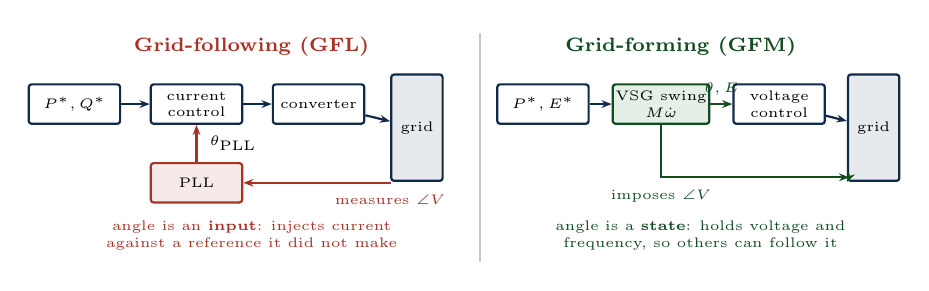
\begin{tikzpicture}[
  font=\tiny,
  blk/.style={draw=pnavy,thick,fill=white,rounded corners=1pt,
              minimum width=1.16cm,minimum height=0.5cm,align=center,inner sep=1pt},
  pll/.style={blk,draw=pred,fill=pred!10},
  vsg/.style={blk,draw=pgreen!60!black,fill=pgreen!12},
  grid/.style={draw=pnavy,thick,fill=pnavy!10,rounded corners=1pt,
               minimum width=0.62cm,minimum height=1.35cm,align=center},
  a/.style={-{Stealth[length=1.3mm]},draw=pnavy,thick},
  am/.style={-{Stealth[length=1.3mm]},draw=pred,thick},
  af/.style={-{Stealth[length=1.3mm]},draw=pgreen!60!black,thick},
  ttl/.style={align=center,font=\scriptsize\bfseries}]

% ------------------------------- GFL --------------------------------------
\node[ttl,pred] at (2.25,2.28) {Grid-following (GFL)};
\node[blk] (pq)  at (0.00,1.55) {$P^\ast,Q^\ast$};
\node[blk] (ci)  at (1.55,1.55) {current\\control};
\node[blk] (inv) at (3.10,1.55) {converter};
\node[grid](g1)  at (4.35,1.25) {grid};
\node[pll] (p1)  at (1.55,0.55) {PLL};
\draw[a] (pq) -- (ci);
\draw[a] (ci) -- (inv);
\draw[a] (inv) -- (g1);
% the defining arrow: the angle comes IN from the grid
\draw[am] (g1.south west) |- (p1.east)
  node[midway,below,font=\tiny,pred,yshift=-0.3mm] {measures $\angle V$};
\draw[am] (p1) -- node[right,font=\tiny,xshift=0.4mm]{$\theta_{\mathrm{PLL}}$} (ci);
\node[align=center,font=\tiny,pred] at (2.25,-0.12)
  {angle is an \textbf{input}: injects current\\against a reference it did not make};

% ------------------------------ divider -----------------------------------
\draw[draw=pnavy!25,thick] (5.15,-0.45) -- (5.15,2.45);

% ------------------------------- GFM --------------------------------------
\node[ttl,pgreen!60!black] at (7.70,2.28) {Grid-forming (GFM)};
\node[blk] (pq2) at (5.95,1.55) {$P^\ast,E^\ast$};
\node[vsg] (sw)  at (7.45,1.55) {VSG swing\\$M\dot\omega$};
\node[blk] (vc)  at (8.95,1.55) {voltage\\control};
\node[grid](g2)  at (10.15,1.25) {grid};
\draw[a] (pq2) -- (sw);
\draw[af] (sw) -- node[above,font=\tiny,pgreen!60!black,yshift=-0.2mm]{$\theta,E$} (vc);
\draw[a] (vc) -- (g2);
% the defining arrow: the angle is generated and pushed OUT.
% Explicit coordinate rather than a ($..$) expression: v11.tex:28 loads only
% arrows.meta/positioning/shapes, and needing \usetikzlibrary{calc} would force
% a preamble change for one arrow.
\draw[af] (sw.south) |- (9.84,0.62)
  node[midway,below,font=\tiny,pgreen!60!black,yshift=-0.3mm] {imposes $\angle V$};
\draw[af] (9.84,0.62) -- (g2.south west);
\node[align=center,font=\tiny,pgreen!60!black] at (7.95,-0.12)
  {angle is a \textbf{state}: holds voltage and\\frequency, so others can follow it};
\end{tikzpicture}

\vspace{0.12cm}
\begin{block}{The consequence for this project}
\small
Neither mode is better in general. GFL tracks its dispatch accurately \emph{while a
reference exists}; GFM supplies that reference but carries the island's frequency
and voltage on its own swing state. The engineering question is therefore not
which mode to pick, but \textbf{which converters must form, when, and how many}.
\end{block}
\end{frame}

% ===================== 4. WHAT THE PROJECT SOLVES ========================
% The "what does this fix" slide the owner asked for. Kept as a from/to
% contrast so the contribution is legible without reading the objectives list:
% the alternative to this framework is a FIXED decision made offline, and the
% cost of that is stated rather than implied.
\begin{frame}{What This Project Provides}
\centering
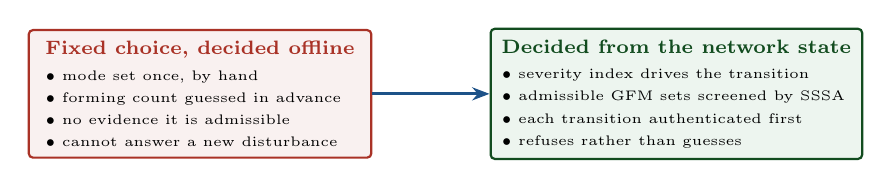
\begin{tikzpicture}[
  font=\scriptsize,
  bad/.style={draw=pred,thick,fill=pred!7,rounded corners=1.5pt,
              minimum width=4.35cm,minimum height=1.62cm,align=left,inner sep=4pt},
  good/.style={draw=pgreen!60!black,thick,fill=pgreen!8,rounded corners=1.5pt,
               minimum width=4.35cm,minimum height=1.62cm,align=left,inner sep=4pt},
  big/.style={-{Stealth[length=2.2mm]},draw=pblue,line width=1.1pt}]
\node[bad]  (l) at (0,0) {%
  \textbf{\color{pred}Fixed choice, decided offline}\\[1.2pt]
  \tiny$\bullet$ mode set once, by hand\\
  \tiny$\bullet$ forming count guessed in advance\\
  \tiny$\bullet$ no evidence it is admissible\\
  \tiny$\bullet$ cannot answer a new disturbance};
\node[good] (r) at (6.05,0) {%
  \textbf{\color{pgreen!60!black}Decided from the network state}\\[1.2pt]
  \tiny$\bullet$ severity index drives the transition\\
  \tiny$\bullet$ admissible GFM sets screened by SSSA\\
  \tiny$\bullet$ each transition authenticated first\\
  \tiny$\bullet$ refuses rather than guesses};
\draw[big] (l) -- (r);
\end{tikzpicture}

\vspace{0.28cm}
\small
\begin{itemize}\setlength{\itemsep}{1.2pt}
  \item One in-house chain --- \textbf{Power Flow} $\rightarrow$ \textbf{SSSA} $\rightarrow$
        \textbf{Time-Domain Simulation} --- on a single shared model, so a screening
        result and a simulated trajectory describe the same system.
  \item Four converters with one common plant and \textbf{selectable GFL/GFM
        controller branches}, switched at run time with current and voltage continuity.
  \item The number of forming units is an \textbf{output} of the network condition,
        not an assumption.
  \item Verified across mode transitions, island support, and SG reconnection
        under an event-driven disturbance chronology.
\end{itemize}
\end{frame}

\end{document}
